\documentclass[10pt,twocolumn,letterpaper]{article}

\usepackage{cvpr}
\usepackage{times}
\usepackage{epsfig}
\usepackage{graphicx}
\usepackage{amsmath}
\usepackage{amssymb}

% Include other packages here, before hyperref.

% If you comment hyperref and then uncomment it, you should delete
% egpaper.aux before re-running latex.  (Or just hit 'q' on the first latex
% run, let it finish, and you should be clear).
\usepackage[pagebackref=true,breaklinks=true,letterpaper=true,colorlinks,bookmarks=false]{hyperref}

% \cvprfinalcopy % *** Uncomment this line for the final submission

\def\cvprPaperID{****} % *** Enter the CVPR Paper ID here
\def\httilde{\mbox{\tt\raisebox{-.5ex}{\symbol{126}}}}

% Pages are numbered in submission mode, and unnumbered in camera-ready
\ifcvprfinal\pagestyle{empty}\fi

\usepackage{color}

\newcommand{\matt}[1]{ \color{red} Matt: #1  \color{black}}
\newcommand{\aneesh}[1]{ \color{blue} Aneesh: #1  \color{black}}
\newcommand{\burak}[1]{ \color{green} Burak: #1  \color{black}}
\newcommand{\emmett}[1]{\color{violet} Emmett: #1  \color{black}}
\begin{document}


%%%%%%%%% TITLE
\title{Multiple Kernelized Correlation Filters based High Speed Target Following}

\author{Burak Uzkent\\
Rochester Institute of Technology\\
{\tt\small bxu2522@@rit.edu}
% For a paper whose authors are all at the same institution,
% omit the following lines up until the closing ``}''.
% Additional authors and addresses can be added with ``\and'',
% just like the second author.
% To save space, use either the email address or home page, not both
\and
YoungWoo Seo\\
Affiliation\\
{\tt\small yseo@autelrobotics.edu}
}

\maketitle
%\thispagestyle{empty}

%%%%%%%%% ABSTRACT
\begin{abstract}

\end{abstract}

%%%%%%%%% BODY TEXT
\section{Introduction}

A practical solution to target-following mode

\begin{itemize}
\item Introduction: Should talk about, at least, motivation of this
  work, brief review of the literature, and contribution
\item Method: Detail the method w.r.t. a diagram of system
  architecture or pseudo code
\begin{itemize}
\item Kernelized Correlation Filter
\item A variant of KCF: Multiple KCF w/ PF
\item Re-detection
\item Estimation of geometry between a target and a drone
\end{itemize}
\item Experiment: Detail the data, and experimental setup; results and findings
\item Conclusion
\end{itemize}

The tracking-by-detection methods have recently emerged as robust,
powerful, and highly discriminative trackers replacing the preceding
generative trackers that focused on only target modeling. Some of the
recent tracking-by-detection algorithms are
Tracking-Learning-Detection \cite{kalal2012tracking}, Multiple
Instance Learning \cite{babenko2009visual}, Correlation Filter based
trackers \cite{bolme2010visual,henriques2015high}, and Struck
\cite{hare2012efficient}. These tracking-by-detection methods train an
object-specific classifier on the fly with the focus of discriminating
the target from the background. Learning an object-specific classifier
in an online manner can better handle challenging scenarios with the
cost of increased complexity. In order to train a classifier, one need
positive and negative samples. Randomly collecting negative samples
from the background area can be one straightforward way of building
training data to train the classifier. However, there can be two
issues in this framework. First, the randomly collected samples can
have large correlation resulting in a weak classifier. Also, such
framework is not feasible for real-time tracking as the number of
samples gradually increases. Most of the tracking-by-detection
algorithms focus on efficient incremental update of a classifier
together with more useful background sampling.

The workflow of our MKCF based long-term target following method can be visualized in fig.~\ref{Workflow_figure}. Summarize what we discuss in the next sections.
\begin{figure*}[!t]
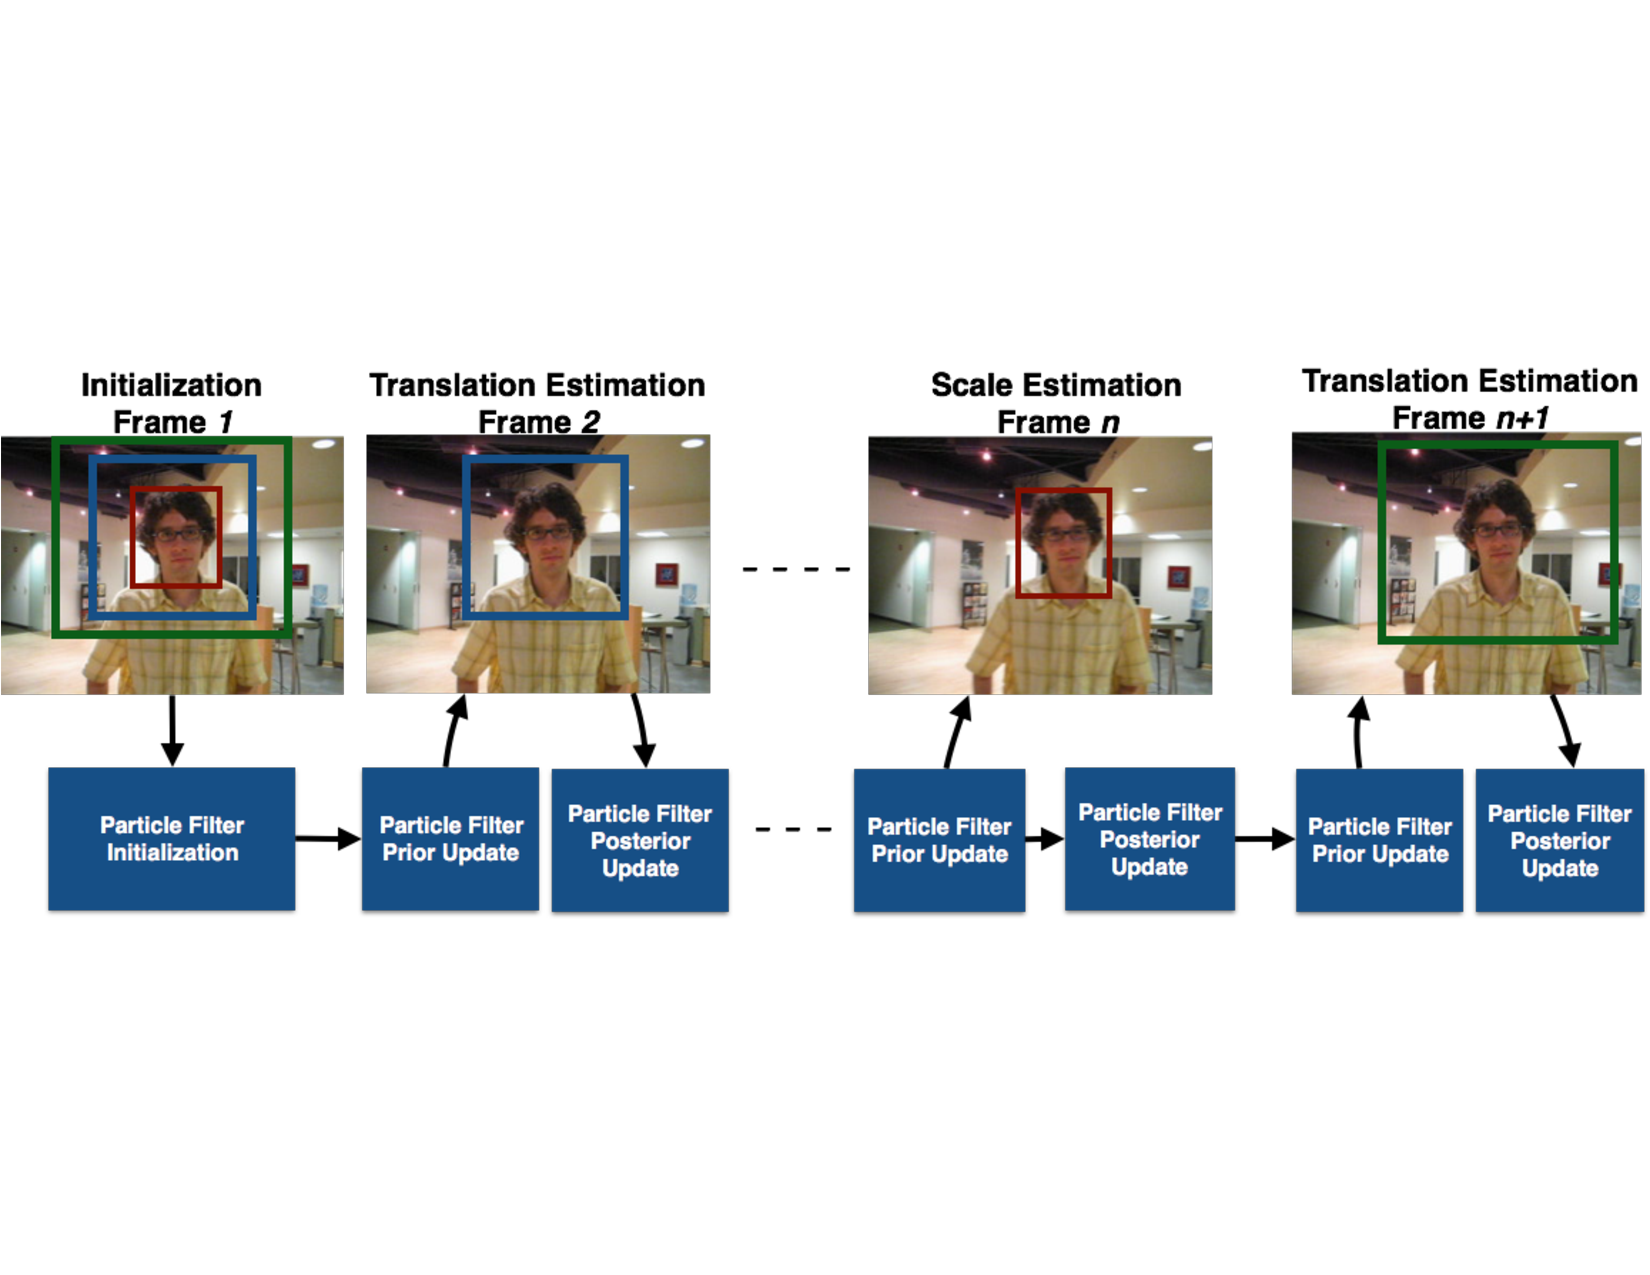
\includegraphics[width=\textwidth]{figures/Workflow_MKCF+PF.pdf}
\caption{The workflow of our Multiple KCF and Particle Filter based tracking method without the track re-detection module.}
\label{Workflow_figure}
\end{figure*}

Frequency domain correlation filter based trackers in the
tracking-by-detection paradigm has recently seen growing popularity
due to its superior computation and robustness to geometric and
photometric variations. The first correlation filter tracker proposed
by \cite{bolme2010visual} focused on learning and detection in the
frequency domain. The idea was to minimize the sum of squared error in
the frequency domain. Hence, the convolution in the original domain is
avoided, instead, element-wise multiplication is needed in the
frequency domain. This way, it achieved promising performance at 700
Hz. On the other hand, the MOSSE tracker failed in cases with rapidly
changing background as it learns the filter using a single template
and accommodates single channel features. Later on, the MOSSE tracker
was improved by using the circularly shifted background patches in an
efficient way by utilizing the theorem that Discrete Fourier Transform
of a circulant matrix gives us diagonalized circulant matrix
\cite{henriques2012exploiting,henriques2015high}. In the same work,
the authors integrated kernelization concept into the detection and
learning steps to improve tracking
accuracy. \cite{galoogahi2013multi,henriques2015high} extended the
correlation filter trackers with single channel features to
multi-channel features. They employed the color and shape features in
a simple framework by summing the correlation of the test and learned
feature channels elements. There a few major drawbacks of the
correlation filter trackers although they outperformed the other
discriminative trackers with superior computation. First, due to the
nature of correlation filters it is limited to a region of interest
which is typically 2-3 times larger than the target. Considering a
larger ROI not only increases the computational burden but also leads
to further spatial information loss with the fixed template size. For
this reason, its performance degrades in fast motion cases as the ROI
may not contain the target. Second, the correlation filter lacks scale
adaptation ability since it only estimates the translation of the
target. Later studies focused on improving the latter issue by
proposing scale candidates where each scale is assigned a confidence
by performing detection on the shrinked or enlarged the ROI
\cite{li2014scale,tang2015multi,bibi2015multi,ma2015long}. Another
group of studies employ the part-based correlation filter trackers to
better adapt to the scale changes
\cite{liu2015real,akin2016deformable}. The sensitivity to fast motion
is generally handled in the long-term target tracking framework where
track reinilization module is triggered when the target is lost
\cite{ma2015long,de2015board,li2016monocular}.

The contributions of this study are as follows.
\begin{itemize}
\item We build a highly efficient ($\geq300$ fps) scale adaptive multiple kernelized correlation filter based tracker that outperforms the original KCF implementation with fixed scale framework both in terms of accuracy and performance. The studies following the KCF improved the fixed scale framework by running detection on a number of candidate ROIs to figure out the new scale of the object after estimating the translation of the object. This approach adds additional complexity to the original KCF implementation and drags down the run-time performance from $300$ fps to less than $100$ fps.
\item We integrate the Particle Filter into the Multiple KCFs tracking as an additional filter that can avoid the drift due to one of the correlation filters we employ in our framework.
\item We propose a target re-detection module that can minimize the target loss due to the scale filter that learns the object model using only-object area. Also, the target re-detection step is required to handle severe occlusions, pose variations, illumination changes and fast motion.
\item Since our visual tracker mostly focuses on tracking objects from aerial moving platforms, we design a new robust target-to-camera distance estimation method. This way, a safe distance between the target and the camera-platform can be preserved.
\end{itemize}

\section{Kernelized Correlation Filter Tracker}
\label{KCF}

%--------------
%\section*{Acknowledgements}
%put stuff here for the accepted , but not the ICCV version


\small
\bibliographystyle{ieee}
\bibliography{draft}

\end{document}
